\documentclass[UTF8]{beamer}

\usepackage{ctex}
\usepackage{setspace}
\usepackage{indentfirst}
\usepackage{ulem}
\usepackage{wasysym}
\usepackage{graphicx}
\usetheme{Dresden}

\setlength{\parindent}{1.5em}
\setlength\parskip{.3\baselineskip}

\title{Computational Geometry}

\author{h10}
\date{}

\begin{document}

	\begin{frame}

		\maketitle

	\end{frame}

	\section{Basic concepts}

	\subsection{Point \& Line \& Vector}

	\begin{frame}{Point}

	A point is an exact position or location on a plane surface.

	In two-dimensional Euclidean space, a point is represented by an ordered pair $(x, y)$ of numbers, where the first number conventionally represents the horizontal and is often denoted by $x$, and the second number conventionally represents the vertical and is often denoted by $y$.

	\end{frame}

	\begin{frame}{Line \& Ray \& Line Segment}

	Line : All definitions are ultimately circular in nature since they depend on concepts which must themselves have definitions.

	Ray : Given a line and any point $A$ on it, we may consider $A$ as decomposing this line into two parts. Each such part is called a ray (or half-line) and the point $A$ is called its initial point. The point $A$ is considered to be a member of the ray. Intuitively, a ray consists of those points on a line passing through $A$ and proceeding indefinitely, starting at $A$, in one direction only along the line.

	Line Segment : A line segment is a part of a line that is bounded by two distinct end points and contains every point on the line between its end points. Depending on how the line segment is defined, either of the two end points may or may not be part of the line segment.

	\end{frame}

	\begin{frame}{Vector}

	A vector space consists of arrows in a fixed plane, starting at one fixed point.

	\end{frame}

	\begin{frame}{Cross product \& Dot product}

	Convex product : $a \times b = |a||b| \sin \theta$.

	Dot product : $a \cdot b = |a||b| \cos \theta$.

	\end{frame}

	\subsection{Convex hull}

	\begin{frame}{Convex hull}

	In mathematics, the convex hull or convex envelope of a set $X$ of points in the Euclidean plane or in a Euclidean space (or, more generally, in an affine space over the reals) is the smallest convex set that contains $X$. 

	For instance, when $X$ is a bounded subset of the plane, the convex hull may be visualized as the shape enclosed by a rubber band stretched around $X$.

	\end{frame}

	\begin{frame}{Minkowski addition}

	In geometry, the Minkowski sum (also known as dilation) of two sets of position vectors $A$ and $B$ in Euclidean space is formed by adding each vector in $A$ to each vector in $B$.

	$A + B = \{ a + b | a \in A, b \in B \}$

	Analogously, the Minkowski difference (or geometric difference) is defined as

	$A - B = \{ c | c + B \in A \}$

	\end{frame}

	\begin{frame}{Rotating calipers}

	\url{https://en.wikipedia.org/wiki/Rotating_calipers}

	\href{Rotating_calipers.gif}{\emph{\underline{demo}}}

	\end{frame}

	\begin{frame}{Convex hull of minkowski sum}

	Both $A$ and $B$ are a set of position vectors.

	let $C = A + B$.

	let $A' = Convex\ hull\ of\ A$.

	let $B' = Convex\ hull\ of\ B$.

	let $C' = Convex\ hull\ of\ C$.

	then, we have $|C'| \leq |A'| + |B'|$.

	\end{frame}

	\begin{frame}{Gift wrapping algorithm}

	The gift wrapping algorithm begins with $i=0$ and a point $p_0$ known to be on the convex hull, e.g., the leftmost point, and selects the point $p_{i+1}$ such that all points are to the right of the line $p_i$ $p_{i+1}$. This point may be found in $O(n)$ time by comparing polar angles of all points with respect to point $p_i$ taken for the center of polar coordinates. Letting $i=i+1$, and repeating with until one reaches $p_h=p_0$ again yields the convex hull in $h$ steps. In two dimensions, the gift wrapping algorithm is similar to the process of winding a string (or wrapping paper) around the set of points.

	\href{Gift_wrapping_algorithm.gif}{\emph{\underline{demo}}}

	\end{frame}

	\begin{frame}{Graham scan}

	\url{https://en.wikipedia.org/wiki/Graham_scan}

	\href{Graham_scan.gif}{\emph{\underline{demo}}}

	\end{frame}

	\begin{frame}{Quickhull(Part 1)}

	The algorithm can be broken down to the following steps:

	1. Find the points with minimum and maximum x coordinates, as these will always be part of the convex hull.

	2. Use the line formed by the two points to divide the set in two subsets of points, which will be processed recursively.

	3. Determine the point, on one side of the line, with the maximum distance from the line. The two points found before along with this one form a triangle.

	4. The points lying inside of that triangle cannot be part of the convex hull and can therefore be ignored in the next steps.

	5. Repeat the previous two steps on the two lines formed by the triangle (not the initial line).

	\end{frame}

	\begin{frame}{Quickhull(Part 2)}

	6. Keep on doing so on until no more points are left, the recursion has come to an end and the points selected constitute the convex hull.

	Under average circumstances the algorithm works quite well, but processing usually becomes slow in cases of high symmetry or points lying on the circumference of a circle.

	\href{Quickhull.gif}{\emph{\underline{demo}}}

	\end{frame}

	\subsection{Plane}

	\begin{frame}{Planar graph}

	In graph theory, a planar graph is a graph that can be embedded in the plane, i.e., it can be drawn on the plane in such a way that its edges intersect only at their endpoints. In other words, it can be drawn in such a way that no edges cross each other.

	\end{frame}

	\begin{frame}{Dual graph}

	Given an embedding $G$ of a connected graph in the plane without edge intersections, we construct the dual graph $G^{*}$ as follows: we choose one vertex in each face of $G$ (including the outer face) and for each edge e in $G$ we introduce a new edge in $G^{*}$ connecting the two vertices in $G^{*}$ corresponding to the two faces in $G$ that meet at e. Furthermore, this edge is drawn so that it crosses e exactly once and that no other edge of $G$ or $G^{*}$ is intersected.

	Attention that $G^{**} = G$.

	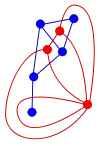
\includegraphics[height=2.3cm]{Dual_graph.png}

	\end{frame}

	\begin{frame}{Point location}

	\url{https://en.wikipedia.org/wiki/Point_location}

	\url{http://blog.miskcoo.com/2015/05/planar-graph-dual-and-point-locate}

	\end{frame}

	\begin{frame}{Half-plane}

	In geometry, a half-space is either of the two parts into which a plane divides the three-dimensional Euclidean space. More generally, a half-space is either of the two parts into which a hyperplane divides an affine space. That is, the points that are not incident to the hyperplane are partitioned into two convex sets (i.e., half-spaces), such that any subspace connecting a point in one set to a point in the other must intersect the hyperplane.

	A half-space can be either open or closed.

	A strict linear inequality specifies an open half-space:

	$a_1x_1 + a_2x_2 + ... + a_nx_n > b$

	A non-strict one specifies a closed half-space:

	$a_1x_1 + a_2x_2 + ... + a_nx_n \ge b$

	\end{frame}

	\begin{frame}{Half-plane intersection}

	\url{http://www.cnblogs.com/huangxf/p/4067763.html}

	\url{https://link.springer.com/article/10.1007/BF02948817?no-access=true}

	\end{frame}

	\section{Exercises}

	\subsection{Problems}

	\begin{frame}{CF \#433 Div.1 E}

	You are given with a centrosymmetric convex hull, split it into several parallelograms.

	$number\ of\ points\ of\ convex\ hull<=2000$

	\end{frame}

	\begin{frame}{distance}

	You are given two groups of Points : group A and graph B.

	Calculate $\max \limits_{u \in A, v \in B} \sqrt{(u_x - v_x)^2 + (u_y - v_y)^2}$.

	$number\ of\ points\ of\ A/B<=100000$

	\end{frame}

	\begin{frame}{MST}

	Problem: \url{MST.png}

	Solution(part1): \url{MST.sol1.png}

	Solution(part2): \url{MST.sol2.png}

	\end{frame}

	\begin{frame}{51nod 1609}

	Problem : \url{http://www.51nod.com/contest/problem.html\#!problemId=1609}

	Solution : \url{http://www.51nod.com/contest/problemSolution.html\#!problemId=1609}

	\end{frame}

	\begin{frame}{51nod 1784}

	Problem : \url{http://www.51nod.com/contest/problem.html\#!problemId=1784}

	Solution : \url{http://www.51nod.com/contest/problemSolution.html\#!problemId=1784}

	\end{frame}

	\begin{frame}{uoj 242}

	Problem : \url{http://uoj.ac/problem/242}

	Solution : \url{http://c-sunshine.blog.uoj.ac/blog/2026}

	\end{frame}

	\begin{frame}{uoj 319}

	Problem : \url{http://uoj.ac/problem/319}

	Solution : \url{noi2017_phantom.pdf}

	\end{frame}

	\section{}

	\begin{frame}

	Thank you for listening.

	\end{frame}

\end{document}

